\documentclass[11pt,a4paper]{article}
\usepackage[utf8]{inputenc}
\usepackage[spanish,es-tabla]{babel}
\usepackage{amsmath}
\usepackage{amsfonts}
\usepackage{amssymb}
\usepackage{graphicx}
\usepackage{natbib}
\usepackage{lineno}
\usepackage{ragged2e}
\usepackage{multicol}
\setlength\columnsep{38pt}
\usepackage{enumerate} 
\usepackage[left=2.8cm,top=2.3cm,right=2.8cm,bottom=2.3cm]{geometry} 
\usepackage{fancyhdr}
\usepackage{url}


\begin{document}
		
		\begin{center}
			\huge \textbf{Metodología Bill Inmon vs Metodología de Kimball} 
		\end{center}
		\vspace{\baselineskip}
		\begin{center}
			
\includegraphics[scale=0.37]{./Imagenes/logo}
		\end{center}
		\vspace{\baselineskip}
		\begin{multicols}{2}
			\small
			\begin{center}
			   	\vspace{\baselineskip}
				Lisbeth Espinoza Caso\\
				2011040667\\                
		        
				\vspace{\baselineskip}
		
				Marlon Xavier Villegas Arando\\
				2015053890\\                

			\end{center}
			\normalsize			
		\end{multicols}
		\vspace{\baselineskip}

		\textbf{\textit{\large Resumen}}\rule[1.5mm]{5mm}{0.1mm}		
		El concepto de Data Warehouse (DW) llegó de la mano de Bill Inmon y Ralph Kimball. Ambos pensaron en un único repositorio de información para poder integrar y explotar información de diversos sistemas fuentes. Pero, más allá de esta generalización conceptual, cada uno decidió hacerlo a su manera. Entonces, veamos qué es lo que propone cada uno de ellos:\\
		\\
		Kimball sugiere utilizar una metodología Bottom-Up, donde la información se extrae de los sistemas transaccionales para ser cargada en diferentes Data Marts cada uno de los cuales son independientes, están modelados en forma dimensional y tienen foco departamental.\\
		\\
		Segun la visión Top-Down de Inmon coincide con el segundo caso de Kimball donde el DW se nutre de un solo ETL, pero en este caso el DW no está modelado dimensionalmente, sino que está en tercera forma normal (3NF). Así, el creador de este modelo entiende que esta forma es mucho más rica y adaptable que el modelo de Kimball. Una vez que tenemos el Data Warehouse generado de esta manera, se pueden crear los datamarts para las áreas de negocio que necesitemos, y además lo podríamos utilizar para cualquier otro tipo de sistema decisional como por ejemplo sistemas expertos, o minería de datos.\\
		
		
		\newpage
		
		\textbf{\textit{\large Abstract}}\rule[1.5mm]{5mm}{0.1mm} 		
		\textit{
			The concept of Data Warehouse (DW) came from the hand of Bill Inmon and Ralph Kimball. Both thought of a single repository of information to be able to integrate and exploit information from different source systems. But, beyond this conceptual generalization, each one decided to do it his own way. Then, let's see what each of them proposes: \\
			\\
			Kimball suggests using a Bottom-Up methodology, where the information is extracted from the transactional systems to be loaded in different Data Marts, each of which are independent, are modeled in dimensional form and have departmental focus. \\
			\\
			According to Inmon's Top-Down vision, it coincides with the second case of Kimball where the DW is nourished by a single ETL, but in this case the DW is not dimensionally modeled, but is in third normal form (3NF). Thus, the creator of this model understands that this form is much richer and more adaptable than the Kimball model. Once we have the Data Warehouse generated in this way, datamarts can be created for the business areas we need, and we could also use it for any other type of decision system such as expert systems, or data mining.
		 }
				
		\vspace{\baselineskip}
		
		\textbf{\textit{\large Keybwords}}\rule[1.5mm]{5mm}{0.1mm} 
		Metodologia, Procesos, Negocios, DataWareHouse
		
						
		\rule{167mm}{0.1mm}
		
		\vspace{\baselineskip}
		
		\section{Introduccion}
		
		Aunque existen otras metodologías o enfoques para la construcción de un DataWarehouse, las más importantes son la propia de Ralph Kimball y la definida por Will Inmon (y su enfoque Enterprise Warehouse o CIF). Es ahí donde llegamos al que parece eterno dilema entre Kimball e Inmon.\\
		\\
		Para entender las diferencias entre ambos enfoques, es necesario en primer lugar tener claro algún concepto, como es la diferencia entre Data Warehouse y Data Mart.
		
			\subsection{Definición de Data Warehouse}
			Un Data Warehouse proporciona una visión global, común e integrada de los datos de la organización, independiente de cómo se vayan a utilizar posteriormente por los consumidores o usuarios. Normalmente en el almacén de datos habrá que guardar información histórica que cubra un amplio período de tiempo. Pero hay ocasiones en las que no se necesita la historia de los datos, sino sólo sus últimos valores, siendo además admisible generalmente un pequeño desfase o retraso sobre los datos operacionales. En estos casos el almacén se llama almacén operacional (ODS, Operational Data Store).
			
			\subsection{Definición de Data Mart}
			Podemos entender un Data Mart como un subconjunto de los datos del Data Warehouse con el objetivo de responder a un determinado análisis, función o necesidad y con una población de usuarios específica. Al igual que en un data warehouse, los datos están estructurados en modelos de estrella o copo de nieve y un data mart puede ser dependiente o independiente de un data warehouse. Por ejemplo, un posible uso sería para el data mining. ¿Qué diferencia existe entonces entre un data mart y un datawarehouse? Su alcance. El data mart está pensado para cubrir las necesidades de un grupo de trabajo o de un determinado departamento dentro de la organización. Es el almacén natural para los datos departamentales. En cambio, el ámbito del data warehouse es la organización en su conjunto. Es el almacén natural para los datos corporativos comunes.
						
		\section{Marco Teórico}
		
			\subsection{Metodología Inmon }
			
			\begin{center}
				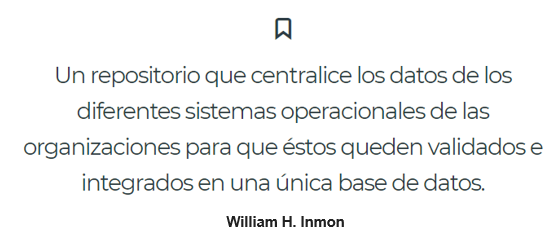
\includegraphics[scale=0.7]{./Imagenes/img01}
			\end{center}		
			
		Según W. H. Inmon (considerado por muchos el padre del Data Warehouse), un Data Warehouse es un conjunto de datos orientados por temas, integrados, variantes en el tiempo y no volátiles, que tienen por objetivo dar soporte a la toma de decisiones.\\
		\\
		Dentro de esta metodología se menciona que la construcción de toda la arquitectura de un Data Warehouse toma bastante tiempo, puesto que su desarrollo inicial está relacionado con necesidades genéricas empresariales, a lo largo del tiempo este tipo de necesidades son cubiertas por el Data Warehouse para más personas por lo que la demanda del uso del Data Warehouse aumenta y esto hace que el performance se vea afectado.\\
		\\
		Es por esto que al llegar a este punto se comienzan a construir segmentos del Data Warehouse que se alimentaran del Data Warehouse y que permitirán tener la información almacenada de manera que esta vaya dirigida a departamentos, con esto se logra disminuir la demanda sobre el Data Warehouse debido a que por ejemplo para este momento en lugar de tener a 100 usuarios requiriendo de manera directa los servicios del Data Warehouse tendré 5 departamentos.[\cite{metodBillInmon1}]
		
		
	
		\begin{enumerate}[A.]
			\item Claves de la arquitectura 
			
			Estas son las claves fundamentales de la arquitectura defendida por Inmon, conocida como ‘Corporate Information Factory (CIF)’, donde el DataWarehouse centraliza todos los datos de la compañía para alimentar, a continuación, pequeños DataMarts temáticos, que serán los puntos de acceso para las herramientas de reporting. En este sentido, cada departamento tendrá su propio DataMart, abastecido con la información del DataWarehouse, listo para su análisis y explotación.
			
			\begin{figure}[!ht]
				\begin{center}
					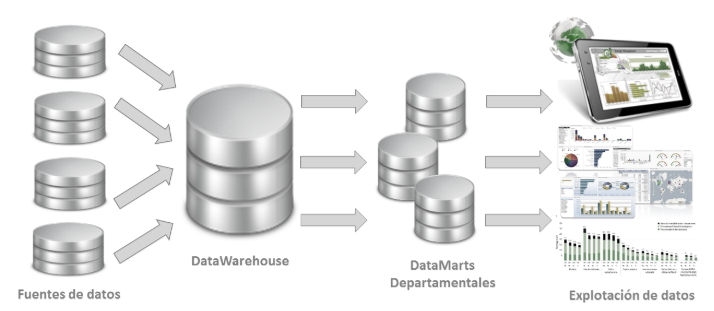
\includegraphics[scale=2.2]{./Imagenes/img03}	
					\caption{Arquitectura Inmon}		
				\end{center}
			\end{figure}
		
			Este enfoque de Inmon suele denominarse una metodología de trabajo ‘Top-Down’, ya que se centra primero en una visión global de la compañía, para ir desmembrándola en pequeños sets de datos departamentales. Así, con esta arquitectura, todos los DataMarts de la organización están conectados al DataWarehouse, evitándose la aparición de incongruencias y anomalías al comparar los datos entre distintos departamentos.
			
			\item Estructura del datawarehouse
			
			En cuanto a la estructura interna del DataWarehouse, para Inmon la prioridad es que el modelo de datos esté construido en tercera forma normal. Por dar una breve explicación de lo que esto significa, el proceso de normalización consiste en aplicar una serie de reglas o normas a la hora de establecer las relaciones entre los diferentes objetos dentro de la base de datos.\\
			\\
			Con este proceso de normalización se consiguen muchos beneficios, como evitar la redundancia de los datos, mantener su integridad referencial, facilitar el mantenimiento de las tablas y disminuir el tamaño de la base de datos. Sin embargo, a diferencia de los DataWarehouse desnormalizados, las consultas exigen el empleo de queries mucho más complejas, lo que dificulta el análisis directo de la información y el uso de las herramientas de reporting. De ahí, la necesidad de construir los DataMarts que, como ya comenté, están basados en modelos dimensionales de estrella o copo de nieve, diseños fácilmente explotables por estas herramientas de análisis de datos.
			
			\begin{figure}[!ht]
				\begin{center}
					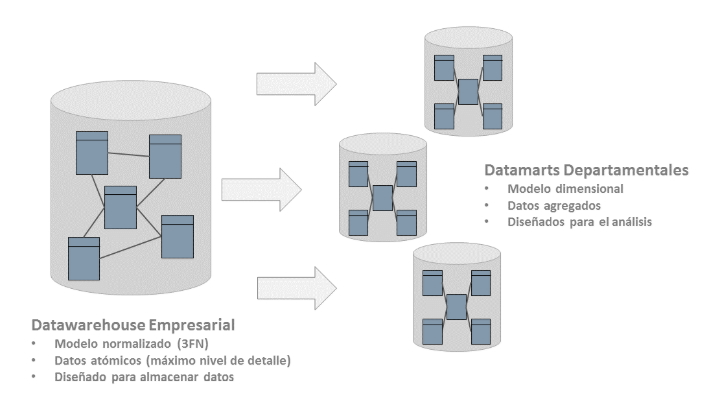
\includegraphics[scale=2.0]{./Imagenes/img04}	
					\caption{Desgloce de la Metodologia}		
				\end{center}
			\end{figure}
			
			\item Implementación del Data Warehouse
			
			\begin{enumerate}[i.]
				\item OLTP\\				
				El primer paso para la implementación de un Data Warehouse es el identificar las fuentes de datos, analizarlas y mapear sus elementos de acuerdo al estándar que hayamos definido. Esto en el orden de tratar de homologar los datos que sea posible para su entrada al Data Warehouse.\\
				
				\item Modelos de Procesos\\
				Se debe tener conocimiento de los procesos que sigue la información y para eso nos sirve el modelo de procesos. Este modelo contiene información como:
					\begin{itemize}
						\item Descomposición funcional
						\item  Diagrama de contexto
						\item Diagrama de flujo de datos
						\item Diagrama de transición de estados
						\item Pseudocódigo\\
					\end{itemize}				
				\item Modelo de datos\\
				El Modelo de datos nos muestra los datos primitivos, tomando en cuenta el elemento tiempo, se plasman los cálculos que se realicen y finalmente se muestran sus relaciones.\\
							
				El Modelo de Datos del Data Warehouse. Los modelos anteriores nos deberán entregar la definición de los sujetos a los que estará orientado el Data Warehouse. Debe venir en 3 perspectivas y son explicadas en la siguiente tabla:
				
					\begin{figure}[!ht]
						\begin{center}
							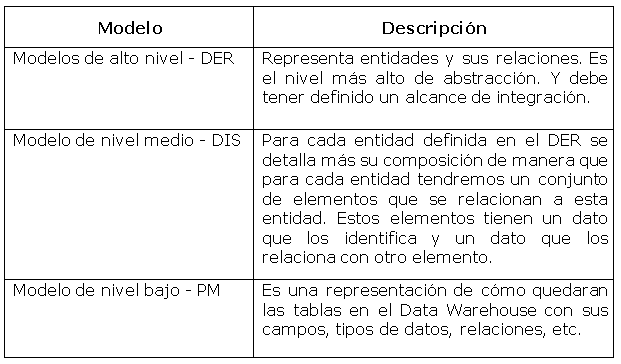
\includegraphics[scale=0.8]{./Imagenes/img02}	
							\caption{Modelado de Datos}		
						\end{center}
					\end{figure}
				
				\item Decisiones sobre el diseño del Data Warehouse\\				
				Una vez que se tiene conocimiento de este modelo se deben tomar ciertas decisiones sobre el diseño del Data Warehouse. Entre estas decisiones tenemos las siguientes:
					\begin{itemize}
						\item Normalización, debemos decidir el grado al que nuestro Data Warehouse.
						\item Granularidad
						\item Particiones
						\item Minería de Datos\\
					\end{itemize}
				
				\item Documento contenidas con estas decisiones\\				
				Al haber tomado estas decisiones, se debe generar un documento que contenga estas decisiones que hemos tomado para la definición del Data Warehouse. Este documento debe contener un concepto de Data Warehouse, una descripción de los sistemas que lo alimentan, como se debe usar el Data Warehouse, como obtener ayuda, responsables, plan de migración, mapeo de datos entre los datos operacionales y el data Warehouse, etc.\\	
				
				\item Metadata\\
				Contiene información sobre nuestro Data Warehouse.\\
				En pocas palabras es un diccionario de datos. Es pieza clave para el mejor aprovechamiento del Data Warehouse. Facilita las tareas de análisis ya que funciona como un índice del contenido del Data Warehouse.
														
			\end{enumerate}
		\item Integración de datos\\
		Implica el implementar procesos ETL que nos permitan extraer la información de los ambientes transacciones para cargarlo dentro del Data Warehouse. Esto puede implicar un cambio en la tecnología, selección de los datos que residirán en el Data Warehouse, cambios de llaves en los objetos, formato de los datos, sumarizaciones, estandarización de nomenclaturas,
		\item Pruebas\\
		Se hacen pruebas al respecto de la implementación del Data Warehouse. Se realizan los ajustes necesarios para poder obtener los resultados esperados en nuestro Data Warehouse.
		\item Programación\\
		Se hacen las programaciones necesarias para que se ejecuten ciertos procesos, para que exista la posibilidad de paralelismo, se administra la Meta Data, índices, particiones, monitoreo, etc
		\item Diseño DSS\\
		Se trabaja sobre un esquema multidimensional para poder generar la información que realmente soporte la toma de decisiones.
		\item Análisis\\
		El tomador de decisiones analiza la información obtenida a partir del DSS.
		\item Requerimientos\\
		A partir del análisis de los datos obtenidos el tomador de decisiones llegue al entendimiento de los requerimientos que tiene su negocio para mejorar.
		
		\end{enumerate}
		El Datawarehouse de Inmon persigue la integración de todos los datos de la compañía, estando orientado hacia el almacenaje de grandes volúmenes de datos, por lo que su estructura interna normalizada se diseña para evitar la redundancia de datos, simplificar las labores de mantenimiento, etc. cuestiones que complican las consultas de la información, requiriendo que los usuarios finales estén mucho más especializados.	
		
		\subsection{Metodologia de Kimball}
	
		La Metodología Kimball, es una metodología empleada para la construcción de un almacén de datos (data warehouse, DW) que no es más que, una colección de datos orientada a un determinado ámbito (empresa, organización, etc.), integrado, no volátil y variable en el tiempo, que ayuda a la toma de decisiones en la entidad en la que se utiliza.\\
		\\
		La metodología se basa en lo que Kimball denomina Ciclo de Vida Dimensional del Negocio (Business Dimensional Lifecycle). Este ciclo de vida del proyecto de DW, está basado en cuatro principios básicos:
		\begin{itemize}
			\item Centrarse en el negocio.
			
			\item Construir una infraestructura de información adecuada.
			
			\item Realizar entregas en incrementos significativos (este principio consiste en crear el almacén de datos (DW) en incrementos entregables en plazos de 6 a 12 meses, en este punto, la metodología se parece a las metodologías ágiles de construcción de software).
			
			\item Ofrecer la solución completa (En este se punto proporcionan todos los elementos necesarios para entregar valor a los usuarios de negocios, para esto ya se debe tener un almacén de datos bien diseñado, se deberán entregar herramientas de consulta ad hoc, aplicaciones para informes y análisis avanzado, capacitación, soporte, sitio web y documentación).[\cite{metodKimball1}]
		\end{itemize}
		
		La construcción de una solución de DW/BI (Datawarehouse/Business Intelligence) es sumamente compleja, y Kimball nos propone una metodología que nos ayuda a simplificar esa complejidad. Las tareas de esta metodología (ciclo de vida) se describen a continuación:\\
		\begin{figure}[!ht]
			\begin{center}
				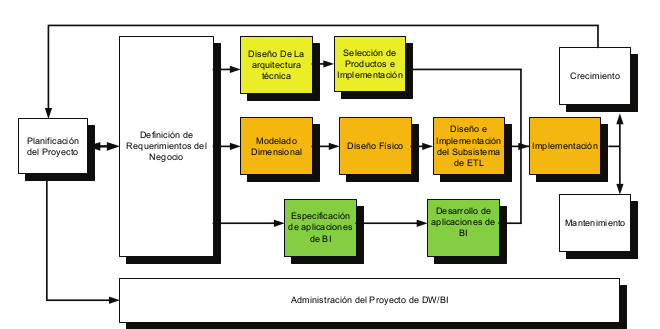
\includegraphics[scale=0.8]{./Imagenes/img05}	
				\caption{Fases de la Metodologia Kimball}		
			\end{center}
		\end{figure}
		\\
		La metodología propuesta por Kimball, esta compuesta por las siguientes fases:
		
		\begin{itemize}
			\item \textbf{Planificación del Proyecto:}  busca identificar la definición y el alcance que tiene el proyecto de DWH. Esta etapa se concentra sobre la definición del proyecto, donde, a nivel de planificación, se establece la identidad del mismo, el personal, desarrollo del plan de proyecto, el seguimiento y la monitorización.
			
			\item \textbf{Definición de los Requerimientos del Negocio:} es un factor determinante en el éxito de un proceso de DWH. Los diseñadores de los Data Warehouse deben tener en claro cuales son los factores claves que guían el negocio para determinar efectivamente los requerimientos y traducirlos en consideraciones de diseño apropiadas.
			
			\item \textbf{Modelado Dimensional:} se comienza con una matriz donde se determina la dimensionalidad de cada indicador para luego especificar los diferentes grados de detalle dentro de cada concepto del negocio.
			
			\item \textbf{Diseño Físico:} se centra en la selección de las estructuras necesarias para soportar el diseño lógico. Un elemento principal de este proceso es la definición de estándares del entorno de la base de datos. La indexación y las estrategias de particionamiento se determinan en esta etapa.
			
			\item \textbf{Diseño y Desarrollo de la presentación de datos:} tiene como principales actividades la extracción, transformación y carga (ETL). Estas actividades son altamente críticas ya que tienen que ver con la materia prima del Data Warehouse que son los datos.
			
			\item \textbf{Diseño de la arquitectura técnica:} en esta fase se deben tener en cuenta tres factores: los requerimientos de negocio, los actuales entornos técnicos, y las directrices técnicas y estratégicas futuras planificadas por la compañía, lo que permitirá establecer el diseño de la arquitectura técnica del entorno del Data Warehouse.[\cite{metodKimball2}]
			
			El proceso de diseño de la arquitectura técnica esta compuesto de 8 pasos:
			
				\begin{enumerate}[1.]
					\item Establecer un grupo de trabajo de arquitectura.
					\item Requisitos relacionados con la arquitectura.
					\item Documento de requisitos arquitectónicos.
					\item Desarrollo de un modelo arquitectónico de alto nivel.
					\item Diseño y especificación de los subsistemas.
					\item Determinar las fases de aplicación de la arquitectura.
					\item Documento de la arquitectura técnica.
					\item Revisar y finalizar la arquitectura técnica.
				\end{enumerate}
			
			\item \textbf{Selección de productos e instalación:} se evalúa y selecciona cuales son los componentes necesarios específicos de la arquitectura (plataforma de hardware, motor de la BD, herramienta de ETL, etc).
			
		\end{itemize}
		
		Luego de realizar la instalación de los componentes previamente evaluados y seleccionados, se recomienda una serie de premisas:
		
		\begin{itemize}
			\item Comprender el proceso de compras corporativas.
			
			\item Elaborar una matriz de evaluación del producto.
			
			\item Realizar la investigación de mercados.
			
			\item Filtrar opciones y realizar evaluaciones más detalladas.
			
			\item Manejo de un prototipo.
			
			\item Selección del producto, instalación y negociación.
			
			\item Especificación de Aplicaciones para usuario finales: se identifican los roles o perfiles de usuarios para los diferentes tipos de aplicaciones necesarias en base al alcance de los perfiles detectados.
			
			\item Desarrollo de aplicaciones para usuario finales: involucra configuraciones de los metadatos y construcción de reportes específicos.
			
			\item Implementación: representa el correcto funcionamiento de la tecnología, los datos y las aplicaciones de usuarios finales accesibles para el usuario del negocio.
			
			\item Mantenimiento y crecimiento: se basa en la necesidad de continuar con las actualizaciones de forma constante para así lograr la evolución de las metas por conseguir.
			
			\item Gestión del proyecto: asegura que todas las actividades del ciclo de vida se lleven a cabo de manera sincronizada.
		\end{itemize}
		
		\begin{enumerate}[A.]
			
			\item Claves de la arquitectura
			
			A este tipo de arquitectura Kimball lo denomina como “Data Warehouse Bus Architecture” y los cuatro pasos fundamentales que se han de seguir para construir este tipo de base de datos son, en primer lugar, la identificación del proceso de negocio que se pretenda estudiar, la definición de la granularidad de los datos, la selección de las dimensiones y atributos y, por último, la identificación de los hechos o métricas.\\
			\\
			El esquema de arquitectura en base a los fundamentos de Ralph Kimball sería el de la siguiente imagen:
			
			\begin{figure}[!ht]
				\begin{center}
					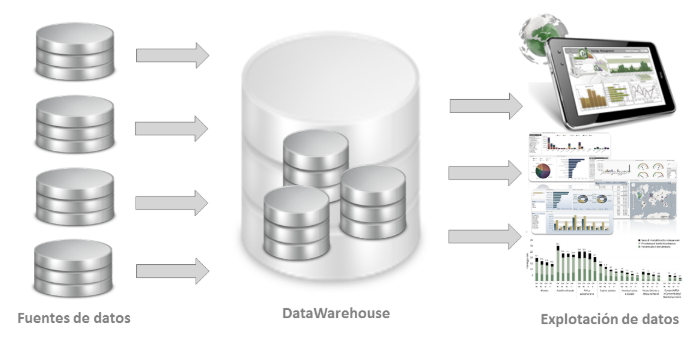
\includegraphics[scale=2.0]{./Imagenes/img06}	
					\caption{Arquitectura Kimball}		
				\end{center}
			\end{figure}
		
			\item Estructura del datawarehouse
			
			A medida que otros departamentos necesiten sus propios datamarts, éstos se irán combinando con el primero manteniendo una metodología de estandarización mediante lo que Kimball denomina “dimensiones conformadas”, que serán las dimensiones comunes entre los diferentes departamentos. La clave radica en que estas dimensiones han de ser compartidas por los distintos datamarts que existan en la organización, garantizándose así la integridad de estos y dando lugar al conglomerado de estructuras que para Kimball conforman el datawarehouse.\\
			\\
			Para lograr este resultado, es importante que estas dimensiones conformadas tengan un diseño consistente y apto para todos los datamarts, de forma que al crearse uno nuevo, reutilice las dimensiones ya definidas, pudiendo incluir o no otras dimensiones nuevas.\\
			\\
			La principal ventaja de este enfoque de almacén de datos es que, al estar formado por pequeños datamarts estructurados en modelos de datos dimensionales (esquemas de estrella o copo de nieve), especialmente diseñados para la consulta y generación de informes, el datawarehouse al completo puede ser explotado directamente por las herramientas de reporting y análisis de datos sin la necesidad de estructuras intermedias.
			
			\begin{figure}[!ht]
				\begin{center}
					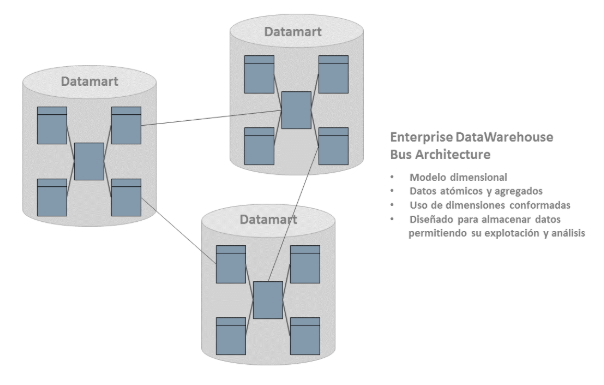
\includegraphics[scale=1.5]{./Imagenes/img07}	
					\caption{Desgloce de la Metodologia Kimball}		
				\end{center}
			\end{figure}
						
		\end{enumerate}
		\newpage
		\section{Comparativa}
		
		Recordando lo presentado en este artículo, el datawarehouse de Kimball está orientado a la consulta de la información, por lo que su estructura interna está especialmente diseñada para garantizar una explotación de los datos rápida y sencilla, no requiriendo usuarios especializados para ello. Por el contrario, el datawarehouse de Inmon persigue la integración de todos los datos de la compañía, estando orientado hacia el almacenaje de grandes volúmenes de datos, por lo que su estructura interna normalizada se diseña para evitar la redundancia de datos, simplificar las labores de mantenimiento, etc. cuestiones que complican las consultas de la información, requiriendo que los usuarios finales estén mucho más especializados.\\
		\\
		Así, podríamos decir que el enfoque de Kimball se ajusta más a proyectos pequeños en los que se persiga un sistema fácilmente explotable y entendible por el usuario y de rápido desarrollo, siendo el modelo de Inmon más apropiado para sistemas complejos de mayor envergadura.\\
		\\
		Todo proyecto tiene sus propias peculiaridades, siendo cada caso único e independiente, por lo que resulta necesario llevar a cabo un estudio de todas ellas antes de decantarnos por una solución u otra, de forma que podamos hacernos una idea sobre qué modelo se ajusta mejor a las condiciones de nuestro proyecto.
		
		\begin{figure}[!ht]
			\begin{center}
				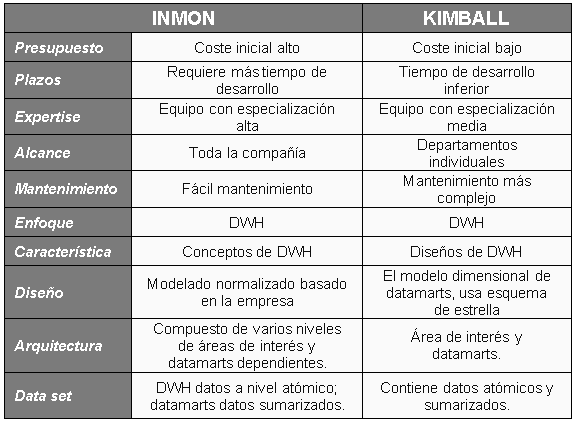
\includegraphics[scale=0.62]{./Imagenes/img08}	
				\caption{Desgloce de la Metodologia Kimball}		
			\end{center}
		\end{figure}
		
		
		\section{Conclusiones}
		
		La metodología Kimball conduce a una solución completa en una cantidad de tiempo relativamente pequeña. Además, debido a la gran cantidad de documentación que se puede encontrar y a los numerosos ejemplos aportados en diferentes entornos, permite encontrar una respuesta a casi todas las preguntas que puedan surgir, sobre todo cuando no se dispone de la experiencia previa necesaria.\\
		\\
		Por otro lado, este tipo de metodología bottom-up permite que, partiendo de cero, podamos empezar a obtener información útil en cuestión de días y después de los prototipos iniciales, comenzar el ciclo de vida normal que nos ofrezca una solución completa de BI.\\
		\\
		Los Data Marts resultantes son fácilmente consultables tanto para los desarrolladores como para los usuarios finales. La relación directa entre los hechos y dimensiones conceden a cualquier usuario la posibilidad de construir consultas muy sencillas, la mayoría de las veces sin tener a mano la documentación de los metadatos.\\
		\\
		La metodología de Kimball es ideal para los primeros pasos de implantación de BI a un cliente, cuando la complejidad de almacenamiento de datos no es demasiado grande y donde la infraestructura del BI se encarga de los datos procedentes de un número limitado de fuentes. Sin embargo, cuando el almacén de datos adquiere complejidad, entonces es peligroso forzar el desarrollo de esta metodología. En el mundo del BI, cuando las cosas adquieren gran complejidad, es el momento de introducir nuevos enfoques al problema, como el propuesto por Inmon.
		
		\bibliographystyle{apalike}
		\bibliography{BIBLIO}
			
		
\end{document}		
